\section{Discretización del modelo tomográfico}

La implementación numérica parte del modelo continuo descrito en los capítulos anteriores, pero reemplaza las funciones por arreglos finitos y las integrales por operaciones discretas. En esta sección se fijan las grillas espaciales, angulares y de detector usadas en todos los experimentos del capítulo.

\subsection*{Discretización del dominio espacial}

Se considera una malla cartesiana uniforme semiabierta en $[-1,1)^2$ de tamaño $N\times N$, con $N=256$. Con paso espacial $h=2/N$, los nodos se escriben como
\[
x_i=\left(i-\frac{N}{2}\right)h,\qquad
y_j=\left(j-\frac{N}{2}\right)h,
\qquad i,j=0,\ldots,N-1.
\]
Así, el índice $N/2=128$ representa exactamente el origen. Esta elección coincide con la convención de \texttt{scikit-image} 0.26.0, que sitúa el eje de rotación de \texttt{radon} en el píxel de índices \texttt{(N//2,N//2)} \cite{scikitimage_radon026}.
El fantoma utilizado es geométrico, asimétrico y está contenido en el disco
\[
x^2+y^2\le R^2,
\qquad R=0.9.
\]
No se usa el fantoma de Shepp--Logan como caso principal, porque se busca un objeto sintético simple con inclusiones de distintas intensidades y posiciones no simétricas.

\subsection*{Grilla angular y detector}

Los ángulos se toman uniformemente en $[0,\pi)$ mediante
\[
\theta_k=k\Delta\theta,
\qquad k=0,\ldots,M-1,
\]
con
\[
M=90,
\qquad \Delta\theta=2^\circ=\frac{\pi}{90}.
\]
Para cada ángulo se genera una proyección discreta, y el conjunto de proyecciones forma un sinograma
\[
g\in\mathbb R^{N_t\times M},
\qquad N_t=256.
\]
La variable del detector se discretiza como
\[
t_\ell=(\ell-N_t/2)\Delta t,
\qquad \ell=0,\ldots,N_t-1,
\]
donde $\Delta t=h=2/N$. El índice $N_t/2=128$ corresponde exactamente a $t=0$ y coincide con el eje del sinograma, que la implementación ubica en \texttt{N\_t//2} \cite{scikitimage_radon026}.

\subsection*{Generación del sinograma}

El sinograma se genera con la rutina \texttt{radon} de \texttt{scikit-image} \cite{vanderwalt2014scikitimage}, usando la opción \texttt{circle=True}. En la versión 0.26.0, esta opción supone que la imagen es nula fuera del círculo inscrito en la malla y hace que el ancho de cada proyección sea igual a la menor dimensión de la imagen \cite{scikitimage_radon026}; por ello se conserva $N_t=N=256$. No describe una geometría de adquisición circular: la adquisición sigue correspondiendo a una geometría de haz paralelo.\\

La definición geométrica continua no se modifica: la recta asociada a $(t,\theta)$ sigue dada por $x\cdot\omega(\theta)=t$, con $\omega(\theta)=(\cos\theta,\sin\theta)$. La implementación debe, sin embargo, distinguir esta convención matemática de la orientación vertical de las matrices digitales, cuyas filas crecen en sentido opuesto al eje cartesiano usual. Esta diferencia se corrige al retroproyectar, sin cambiar la definición de la transformada de Radon.\\

La Figura~\ref{fig:chapter3-phantom-sinogram} muestra el fantoma y el sinograma generado con estos parámetros.

\begin{figure}[htbp]
    \centering
    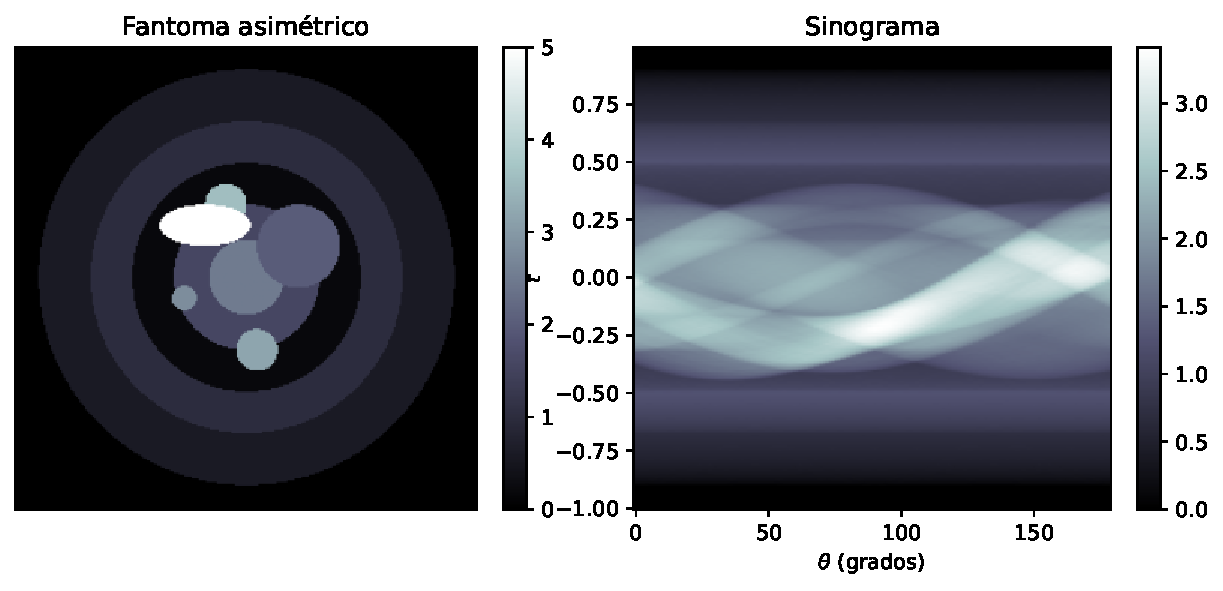
\includegraphics[width=0.92\textwidth]{Figures/Chapter3/phantom_and_sinogram.pdf}
    \caption{Fantoma geométrico utilizado en los experimentos y sinograma generado con $M=90$ ángulos de haz paralelo. El fantoma está contenido en el disco de radio $R=0.9$, y el sinograma constituye el dato de entrada para las reconstrucciones posteriores.}
    \label{fig:chapter3-phantom-sinogram}
\end{figure}

Esta discretización es suficiente para estudiar el comportamiento relativo de los filtros considerados. Existen formulaciones formales de transformadas de Radon discretas, como la de Beylkin \cite{beylkin1987}, pero la implementación de esta tesis corresponde a un modelo muestreado basado en sinogramas generados numéricamente y no a una implementación exacta de dicha transformada discreta. Los errores introducidos por interpolación, muestreo espacial y muestreo angular forman parte del modelo numérico evaluado y no se corrigen mediante ajustes posteriores de amplitud \cite{kak_slaney1988,natterer2001}.
